\documentclass[12pt, letterpaper]{article}

% Font
\usepackage[MnSymbol]{mathspec}
\setmainfont{Minion Pro}
\setmathsfont(Digits,Latin,Greek)
[Numbers={Lining,Proportional}]{Minion Pro}
\usepackage{microtype}

% Format
\usepackage[letterpaper, margin = 1in]{geometry}
\setcounter{secnumdepth}{2}
\renewcommand{\thesection}{\Alph{section}} 
\usepackage{titlesec}  
\titleformat*{\section}{\centering\normalfont\Large\bfseries}

% Links
\usepackage[colorlinks = true, linkcolor = black, urlcolor = black, citecolor = black]{hyperref} 

% Figures
\usepackage{graphicx}
\usepackage[labelfont = bf, font = small, labelsep = newline, singlelinecheck = false]{caption}
\renewcommand{\thefigure}{S\arabic{figure}}
\renewcommand{\thetable}{S\arabic{table}}

% Tables
\usepackage{booktabs}
\usepackage{xltabular}

% Lists
\providecommand{\tightlist}{%
  \setlength{\itemsep}{0pt}\setlength{\parskip}{0pt}}

% References
\newenvironment{CSLReferences}[2]{}{}

% Frontmatter
\title{ Supplemental Online Materials:\\\textit{Double Standards in
Judging Collective Action} }
\author{  }

\begin{document}

\maketitle

\hypertarget{scale-development}{%
\section{Scale Development}\label{scale-development}}

\hypertarget{study-1}{%
\subsection{Study 1}\label{study-1}}

In Study 1, we compiled a list of collective actions from participants'
responses and other sources. To that end, we recruited 60 participants
from the Prolific subject pool, all of whom were citizens of the UK or
the US. To increase the socioeconomic diversity of our sample, we
recruited 30 non-students without a university degree, 15 non-students
with a university degree, and 15 current university students.
Participants first read an accessible description of collective action:

\begin{quote}
Society is not only made up of individuals, but consists of `social
groups' to which these individuals belong. Each person lives in a place,
has a job (or not) at an organisation, is a fan of a specific sports
club, has a religion, or belongs to any number of other such groups.
Individuals often act in ways to promote the interests of the social
groups to which they belong.
\end{quote}

\begin{quote}
For example, the workers in a factory might want to get paid more. They
might go on a strike to reach that goal. Students at a university might
want to prevent an increase in tuition fees. They might hand out flyers
or occupy a building to reach that goal. Other groups might want to
protest against police violence. They might block traffic on a road to
make others aware of this issue.
\end{quote}

\noindent Participants were then asked to name at least five (and up to
ten) actions that fit that description and were encouraged to think of
actions that vary in how acceptable or unacceptable they are (in their
opinion):

\begin{quote}
Please think of other actions that members of a social group (or social
groups as a whole) might take to promote their group's interests or
goals. Please name at least 5 actions that fit the description above.
You can name up to 10 actions if you want to. Please try to think of
actions that vary in how acceptable or unacceptable they are (in your
opinion).
\end{quote}

\noindent After naming at least five actions, participants sorted their
responses into actions that, across a range of situations, were ``always
acceptable'', ``sometimes acceptable'', and ``never acceptable'':

\begin{quote}
On the left, you see the actions you have named on the previous page.
Think about each action. Can you think of situations in which this
action is an acceptable means to advance a group's goals or interests?
Can you think of situations in which this action is not an acceptable
means to advance a group's interests?
\end{quote}

\noindent Participants named between 5 and 10 actions
(\(\textit{Mdn} = 7\)). Participants named more actions that they
considered always acceptable (\(\textit{Mdn} = 3\)) than actions they
considered sometimes (\(\textit{Mdn} = 2\)) or never
(\(\textit{Mdn} = 1\)) acceptable. We recoded participants' responses
into a smaller set of unique collective actions. We then supplemented
the resulting list of actions with collective actions from the
psychological and political science literature (e.g., Sharp, 1973). This
process resulted in 72 actions that we expected to vary in how
acceptable most people would find them to be.

\hypertarget{study-2}{%
\subsection{Study 2}\label{study-2}}

In Study 2, we measured how acceptable participants judged the actions
from Study 1 to be and applied item response theory to develop an
instrument to capture double standards in judging collective action. We
recruited 158 participants (\(\textit{Mdn} = 30\) years, age range:
18--68 years; 103 women, 52 men, 2 other, 1 prefer not to say) from the
Prolific subject pool, all of whom were citizens of the UK or the US. To
increase the socioeconomic diversity of our sample, we recruited 80
non-students without a university degree, 37 non-students with a
university degree, and 41 current university students. We excluded 15
participants who failed an attention check, leaving a final sample of
143 participants for our analyses.

Participants first read an accessible description of collective action:

\begin{quote}
Society is not only made up of individuals, but consists of `social
groups' to which these individuals belong. Each person lives in a place,
has a job (or not) at a firm or organisation, has a religion (or not),
is part of a political party, or belongs to any number of other groups
like these.
\end{quote}

\begin{quote}
Individuals often act in ways to promote their group's interest. For
example, individuals might want people like them to get paid more.
Members of a group might take various kinds of actions (for example, go
on a strike).
\end{quote}

\noindent Participants were then asked to ``suppose that one or more
members of a group took the following action to advance a cause in their
group's interest'' and were presented with one of the actions from Study
1. Participants answered several questions about the protest action.
First, they rated how disruptive, violent, and extreme they considered
this action to be (1 = \emph{not at all}, 4 = \emph{very}). Second, they
were asked to think of a range of different causes and circumstances,
and to rate how often this action would be an acceptable means for a
group to advance one of these causes (1 = \emph{never}, 2 =
\emph{rarely}, 3 = \emph{sometimes}, 4 = \emph{often}, 5 =
\emph{always}). Finally, they rated how positive or negative they felt,
in general, about this action (1 = \emph{very positive}, 5 = \emph{very
negative}). Each participant answered these questions for 20 of the 72
actions from Study 1 so that each action was rated by 29--53
participants.

We estimated a graded response model (Bürkner, 2021; Samejima, 1997), an
item response theory model for ordinal response variables, for
participants' ratings of how often an action would be an acceptable form
of collective action. For each participant \(j\), the model estimated
their unique propensity (\(\theta_j\)) to consider collective actions
acceptable in more situations. For each item \(i\), the model estimated
four acceptability thresholds (\(\beta_{ik}\)), separating the five
response options, and one discrimination parameter (\(\alpha_i\))
indicating how well the item differentiates between participants with
different propensities to consider collective actions acceptable. We
estimated the model in \emph{CmdStanR} using similar prior distribution
as in Experiment 1. We used an induced Dirichlet prior (Betancourt,
2019) for the item-specific difficulty thresholds.

Table S1 shows each protest action's information and discrimination
parameters as well as the proportions of participants choosing each
answer option. Table S2 shows participants' averaged ratings of how
acceptable, disruptive, violent, extreme, and negative they considered
each action to be. Table S3 shows that all five ratings were strongly
correlated across actions and participants.

Figure \ref{fig:s1} shows the scale information curves for scales
composed of, respectively, the 1--72 most informative and discriminating
protest actions. We selected the 25 most informative actions to
construct the final scale to be used in Experiments 1--3. While adding
more actions to the scale would have improved the information provided
by the instrument, the added benefit of each additional action included
in the scale would have been small (see Figure \ref{fig:s1}). We limited
the number of protest actions to 25 so as to not overwhelm participants
and to prevent satisficing. Tables A1, B1, and C1 list the protest
actions used in Experiments 1--3.

\begin{figure*}[!t]
\centering
\caption{Scale information curves for scales composed of the 1--72 most informative and discriminating protest actions}
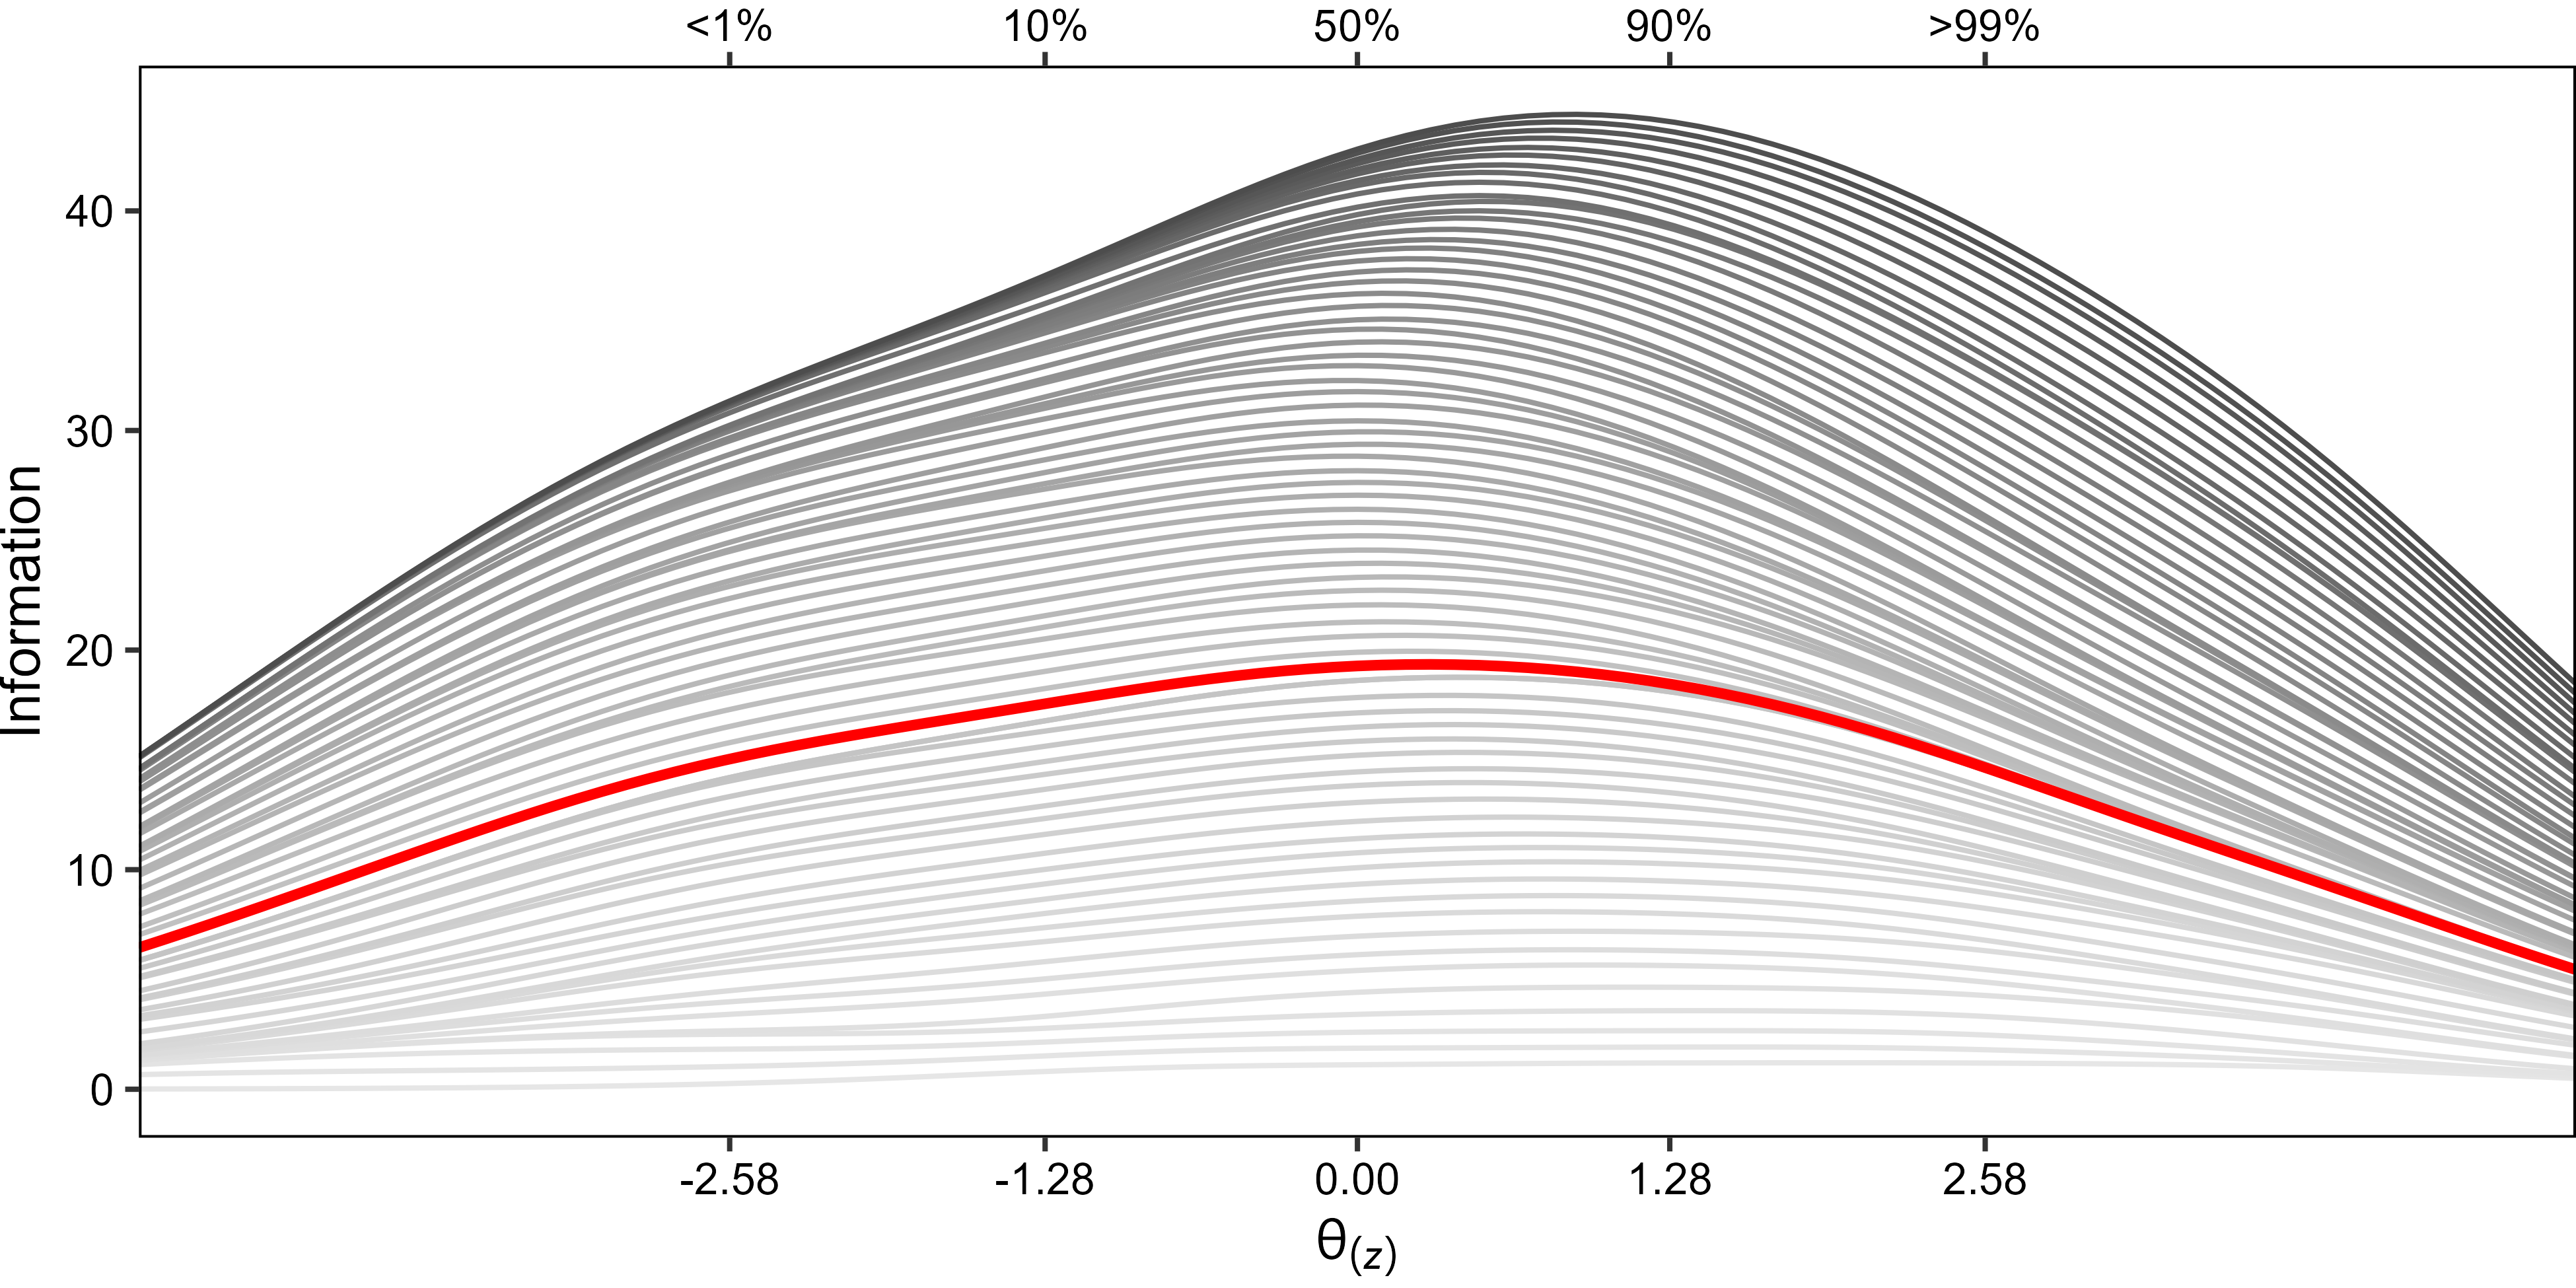
\includegraphics[scale=1]{../Scale Development/figures/figure-s1}
\caption*{\textit{Note.} The information curve for the final scale of 25 actions is highlighted in red. As in Figure 1, $\theta_{(z)}$ follows a standard normal distribution and is shown as both $z$-scores (bottom) and percentiles (top).}
\label{fig:s1}
\end{figure*}

\hypertarget{experiment-1}{%
\section{Experiment 1}\label{experiment-1}}

\hypertarget{method}{%
\subsection{Method}\label{method}}

\hypertarget{procedure}{%
\subsubsection{Procedure}\label{procedure}}

We used a two-step process to recruit participants who satisfied our
preregistered inclusion criteria.

First, we recruited a larger pool of 875 participants. Of these, 475
participants did not have a university degree and placed themselves on
the bottom three ranks of the subjective socio-economic status ladder
(\emph{lower-status group}) and 400 participants had at least an
undergraduate degree and placed themselves on the top four ranks of the
subjective socio-economic status ladder (\emph{higher-status group}).
Participants completed a screening survey in which they, among other
questions, answered whether they considered either their current job or
the jobs they had had in the past or would have in the future to be a
working-class job or a middle-class/professional job (1 =
\emph{working-class job}, 2 = \emph{middle-class/professional job}, 3 =
\emph{neither}). Before answering this question, participants read the
following explanation:

\begin{quote}
The workforce is often divided into two kinds of jobs. What we call
working-class jobs are jobs done by skilled, semi-skilled, unskilled
manual workers or by casual workers. These jobs do not usually require a
university degree. What we call middle-class or professional jobs are
administrative, managerial, or other jobs that usually require a
university degree.
\end{quote}

\noindent As preregistered, we excluded participants from the
lower-status group who had responded ``middle-class/professional job''
or ``neither'' to this question; we excluded participants from the
higher-status group who had responded ``working-class job'' or
``neither'' to this question. This left 687 participants for the next
step of the selection procedure.

Second, we set out to recruit 500 participants from the remaining 687
participants, 250 from the lower-status group and 250 from the
higher-status group. After giving their informed consent, participants
were randomly assigned to read a vignette about a government bill
affecting either people in working-class jobs (\emph{lower-status
protesters}) or people in professional jobs (\emph{higher-status
protesters}). Participants in both conditions were instructed to
carefully read the vignette and to try to imagine what it would be like
if this situation was real. Participants in the lower-status protesters
condition then read the following introduction:

\begin{quote}
The government, though not necessarily the current government, is going
to introduce a bill that will mostly affect people in working-class
jobs. Working-class jobs, in this case, are jobs done by skilled,
semi-skilled, unskilled manual workers or by casual workers. These are
jobs that do not usually require a university degree. Other jobs are
unlikely to be affected.
\end{quote}

\noindent Participants in the higher-status protesters condition instead
read the following introduction:

\begin{quote}
The government, though not necessarily the current government, is going
to introduce a bill that will mostly affect people in professional jobs.
Professional jobs are administrative, managerial, or other jobs that
usually require a university degree. Other jobs are unlikely to be
affected.
\end{quote}

\noindent Participants in the two conditions then read this almost
identically worded paragraph:

\begin{quote}
This government measure would make it easier for companies to hire
workers during economic growth and to lay off workers during an economic
crisis. As a consequence, companies would be able to fire employees with
little notice and without giving a reason. Trade unions are opposed to
the measure. They argue that the bill would compromise job security, and
prevent employees from challenging harassment or other abuse without the
fear of being fired. People in {[}working-class/professional{]} jobs are
particularly at risk, and there is a rise in tension and outrage among
them.
\end{quote}

After reading the vignette, participants responded to the other measures
(in the order in which they are presented in the main text). On the
final page, we reminded participants that they had read about a bill
that the government planned to introduce and that some people objected
to. As an attention check, we then asked participants to recall who the
people most affected by this measure were. As preregistered, we excluded
all participants who did not respond with an accurate description of the
group they had read about.

\hypertarget{experiment-3}{%
\section{Experiment 3}\label{experiment-3}}

\hypertarget{method-1}{%
\subsection{Method}\label{method-1}}

\hypertarget{measures}{%
\subsubsection{Measures}\label{measures}}

We included additional measures not used in the analyses reported in
this paper.

We included a three-item measure of moral conviction (Ryan, 2014) that
assessed to what extent participants' feelings about restricting or
banning abortion were, for example, connected to their core moral
beliefs or convictions (1 = \emph{not at all}, 5 = \emph{very much}).

We measured gender-related system-justifying beliefs with eight items
(adapted from Jost \& Kay, 2005), for example, ``in general, relations
between men and women are fair'' (1 = \emph{strongly disagree}, 7 =
\emph{strongly agree}; McDonald's \(\omega = .93\)). A confirmatory
factor analysis model in which all items loaded onto a single factor
showed acceptable fit,
\(\chi^2 (20) = 111.90; \text{CFI} = 0.97; \text{TLI} = 0.95; \text{RMSEA} = 0.09, [0.08, 0.11]\).

We measured moral concerns with the 36-item moral foundations
questionnaire (MFQ-2, Atari et al., 2023) which assesses to what extent
participants endorse concerns about care, equality, proportionality,
loyalty, authority, and purity (e.g., ``I believe chastity is an
important virtue.''; 1 = \emph{does not describe me at all}, 5 =
\emph{describes me extremely well}). We embedded three further attention
checks within the questionnaire (e.g., ``To show that you are paying
attention and giving your best effort, please select `moderately
describes me'.'').

\hypertarget{reanalyses-without-exclusions}{%
\section{Reanalyses Without
Exclusions}\label{reanalyses-without-exclusions}}

We replicated the analyses for Experiments 1-3 using the complete data
without excluding participants based on the (preregistered) exclusion
criteria.

\hypertarget{experiment-1-1}{%
\subsection{Experiment 1}\label{experiment-1-1}}

\begin{figure*}[!t]
\centering
\caption{Results from the preregistered (\textbf{A}) and non-preregistered (\textbf{B}) analyses for Experiment 1 without exclusions}
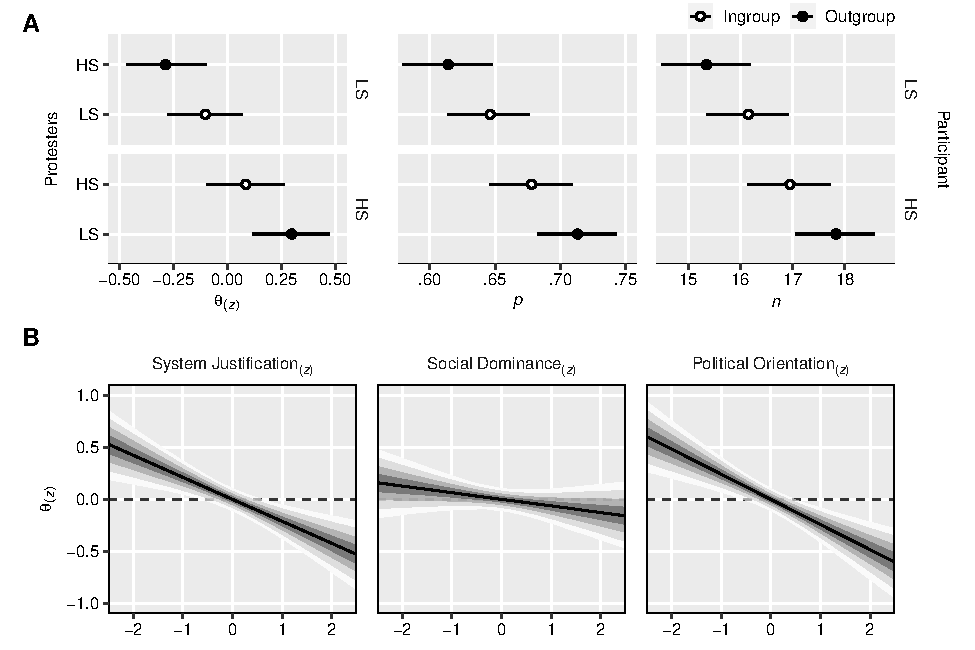
\includegraphics[scale=1]{../Experiment 1/figures/figure-s2}
\caption*{\textit{Note.} HS = Higher Status, LS = Lower Status. $\theta_{(z)}$ is the \textit{z}-standardized tendency to consider more controversial actions acceptable means of protest. (\textbf{A}) $p$ and $n$ are, respectively, the predicted proportion and number of actions a participant would consider acceptable means of protest in each condition. Bars enclose the 95\% most plausible estimates. (\textbf{B}) Ribbons enclose, from the darkest to the lightest shade, the 50\%, 80\%, 95\%, and 99\% most plausible estimates.}
\label{fig:s2}
\end{figure*}

Figure \ref{fig:s2} (A) shows estimates for each combination of the
protesters' and the participants' group membership. Overall, we found
that participants' responses depended on both the protesters' and the
participants' group status---but not in the directions predicted by our
hypotheses. Contradicting our first hypothesis, participants did not
consider protest actions performed by their ingroup to be more
acceptable, on average, than the same actions performed by the relevant
outgroup (Cohen's \(d = -0.01, [-0.20, 0.16]\)). Instead, we found that
participants from higher-status backgrounds considered protest actions
performed by both lower-status (\(d = 0.40, [0.15, 0.66\){]}) and
higher-status (\(d = 0.37, [0.10, 0.63]\)) protesters to be, on average,
more acceptable than participants from lower-status backgrounds.
Contradicting our second hypothesis, participants considered protest
actions performed by higher-status protesters to be less acceptable, on
average, than the same actions performed by lower-status protesters
(\(d = -0.20, [-0.37, -0.02]\)).

Figure \ref{fig:s2} shows (B) the \(z\)-standardized propensity to
consider more controversial protest actions acceptable as a function of
the three ideological orientation variables. We found that participants
who reported a more right-wing political orientation
(\(\beta_{xy} = -0.24, [-0.34, -0.15]\)) and who expressed more
agreement with system-justifying beliefs
(\(\beta_{xy} = -0.21, [-0.31, -0.12]\)) tended to find fewer collective
actions to be acceptable. In contrast, we found that, after controlling
for the other two variables, social dominance orientation was not
associated with participants' judgments about how acceptable various
collective actions are (\(\beta_{xy} = -0.06, [-0.16, 0.03]\)). Overall,
these findings suggest that people who are right-wing and endorse
system-justifying beliefs tend to find various collective actions to be
less acceptable than people who are left-wing and do not endorse
system-justifying beliefs.

\hypertarget{experiment-2}{%
\subsection{Experiment 2}\label{experiment-2}}

\hypertarget{preregistered-analyses}{%
\subsubsection{Preregistered Analyses}\label{preregistered-analyses}}

\begin{figure*}[!t]
\centering
\caption{Results from the preregistered analyses for Experiment 2}
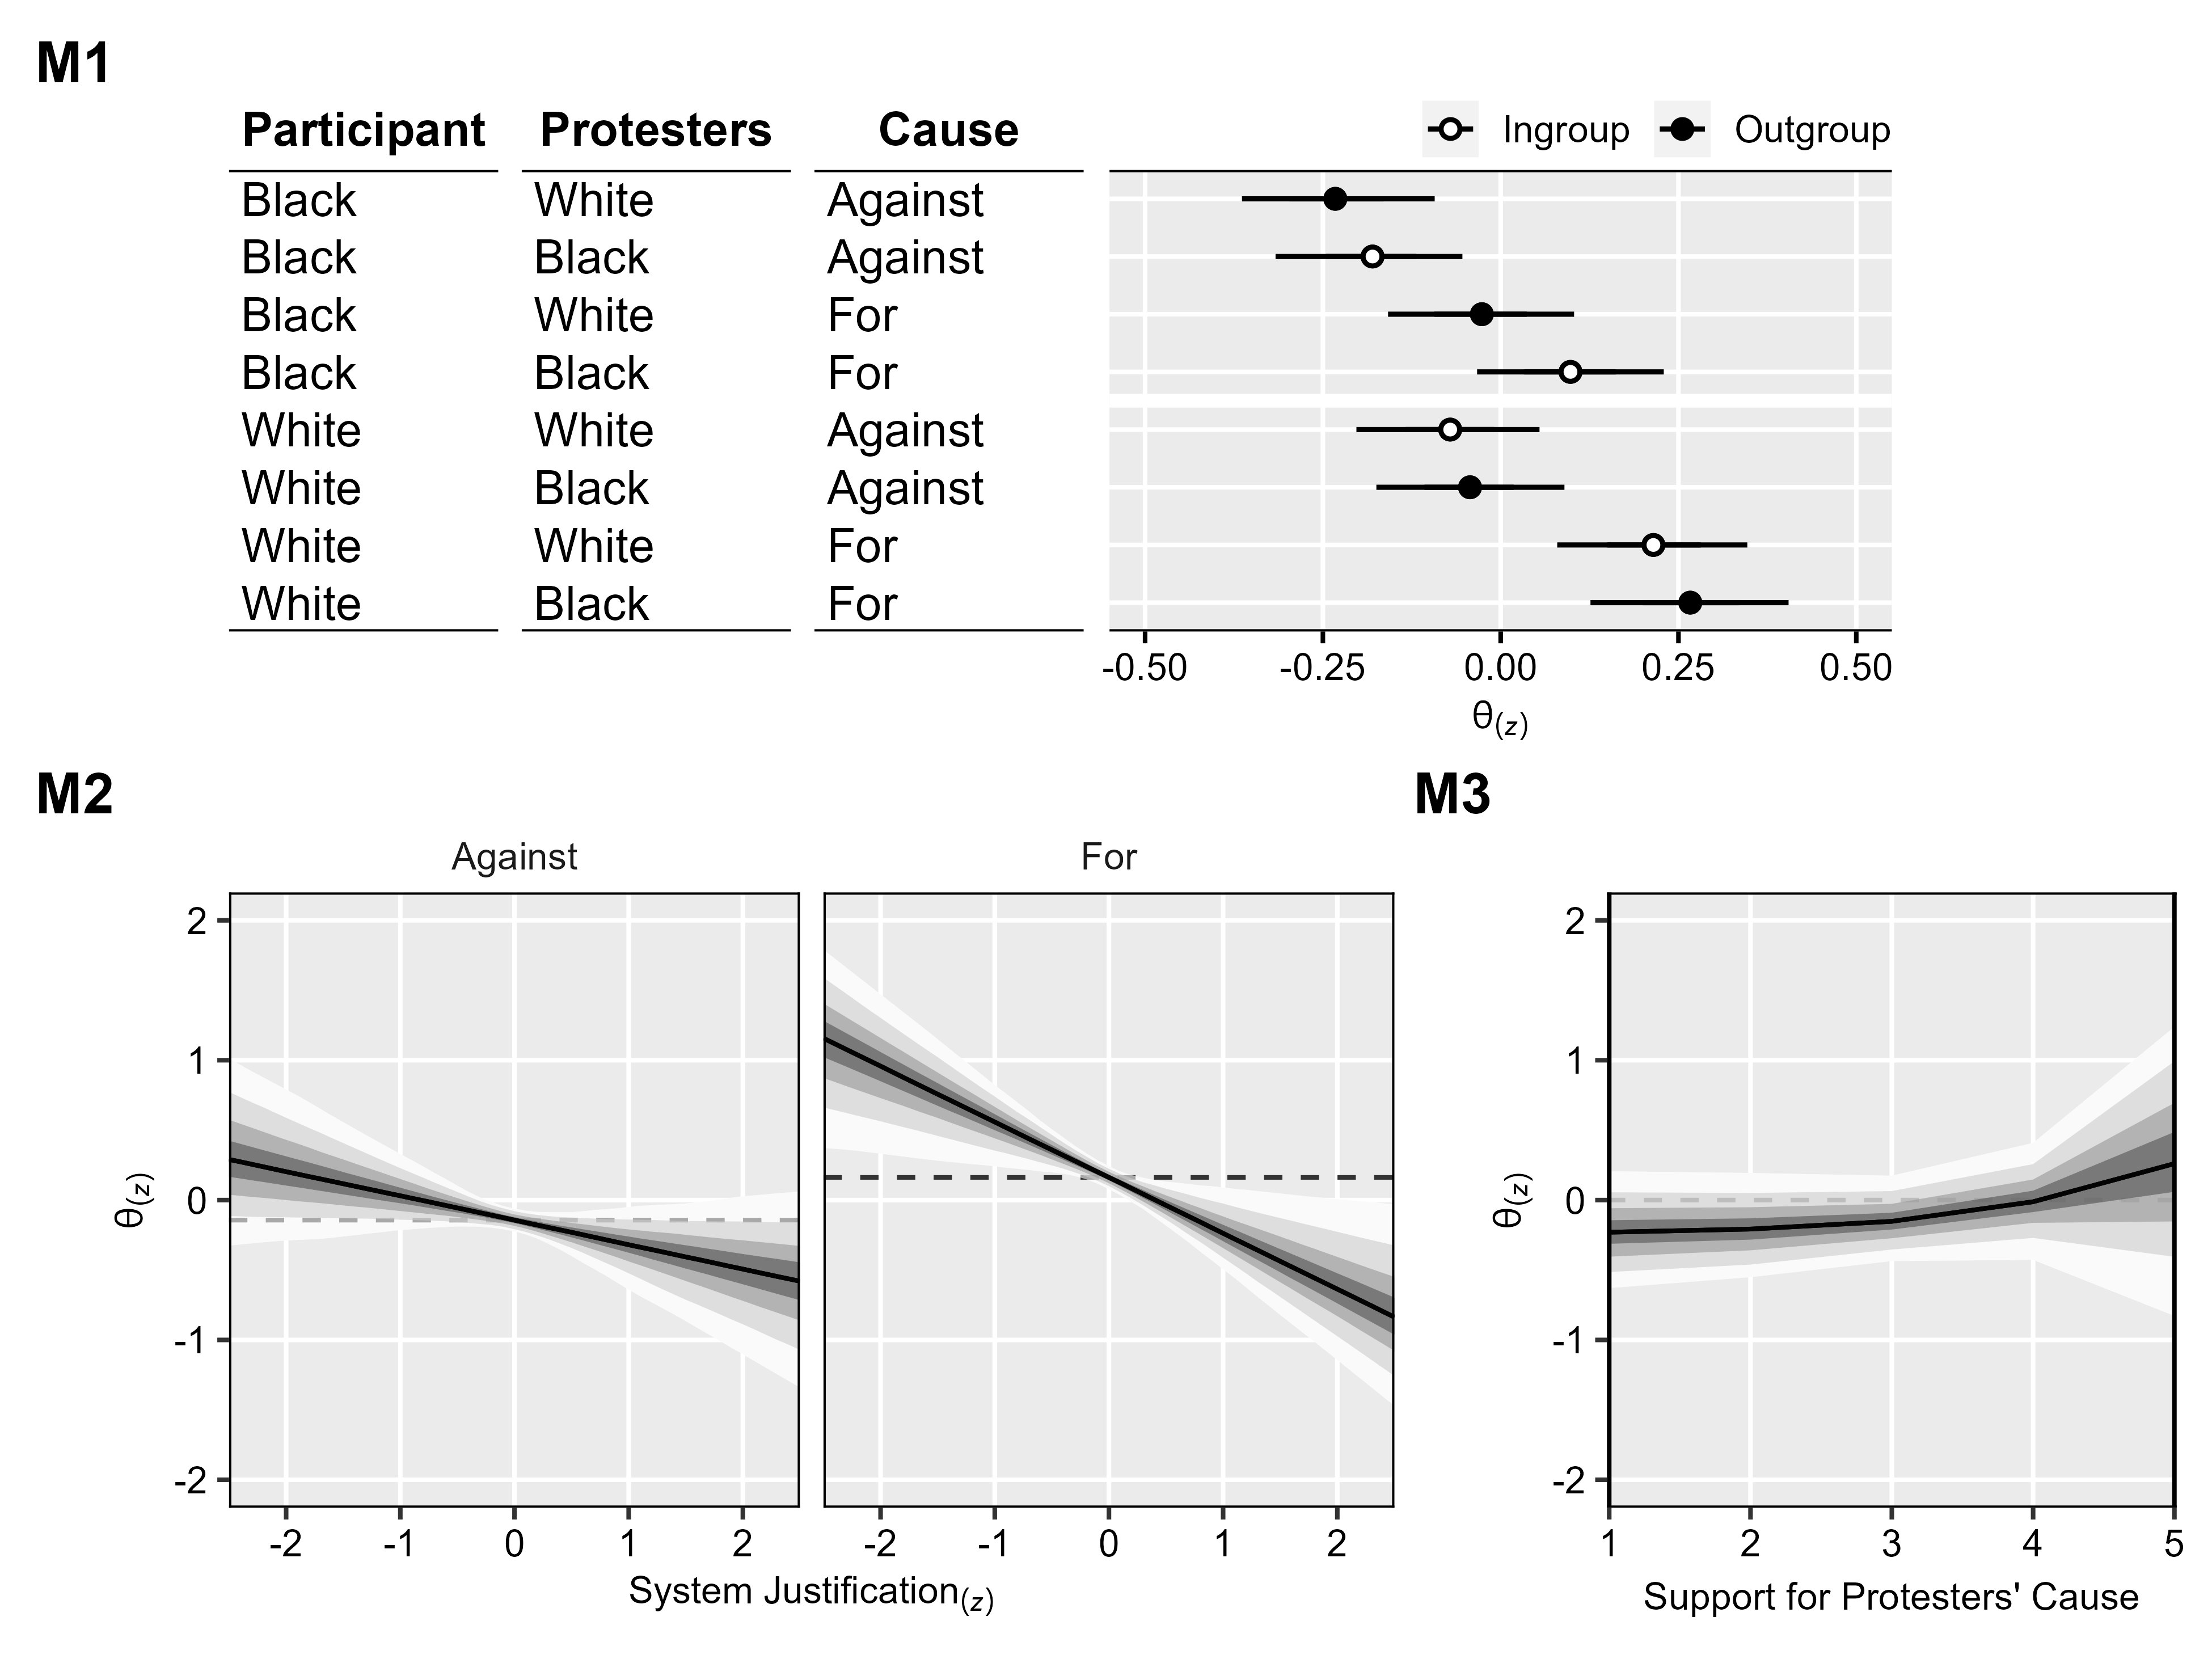
\includegraphics[scale=1]{../Experiment 2/figures/figure-s3}
\caption*{\textit{Note.} Against = Protesters oppose defunding the police. For = Protesters support defunding the police. $\theta_{(z)}$ is the \textit{z}-standardized tendency to consider more controversial actions acceptable means of protest. Ribbons enclose, from the darkest to the lightest shade, the 50\%, 80\%, 95\%, and 99\% most plausible estimates.}
\label{fig:s3}
\end{figure*}

\begin{figure*}[!t]
\centering
\caption{Predictions from the preregistered (system justification) and non-preregistered (political orientation) analyses for Experiment 2 without exclusions}
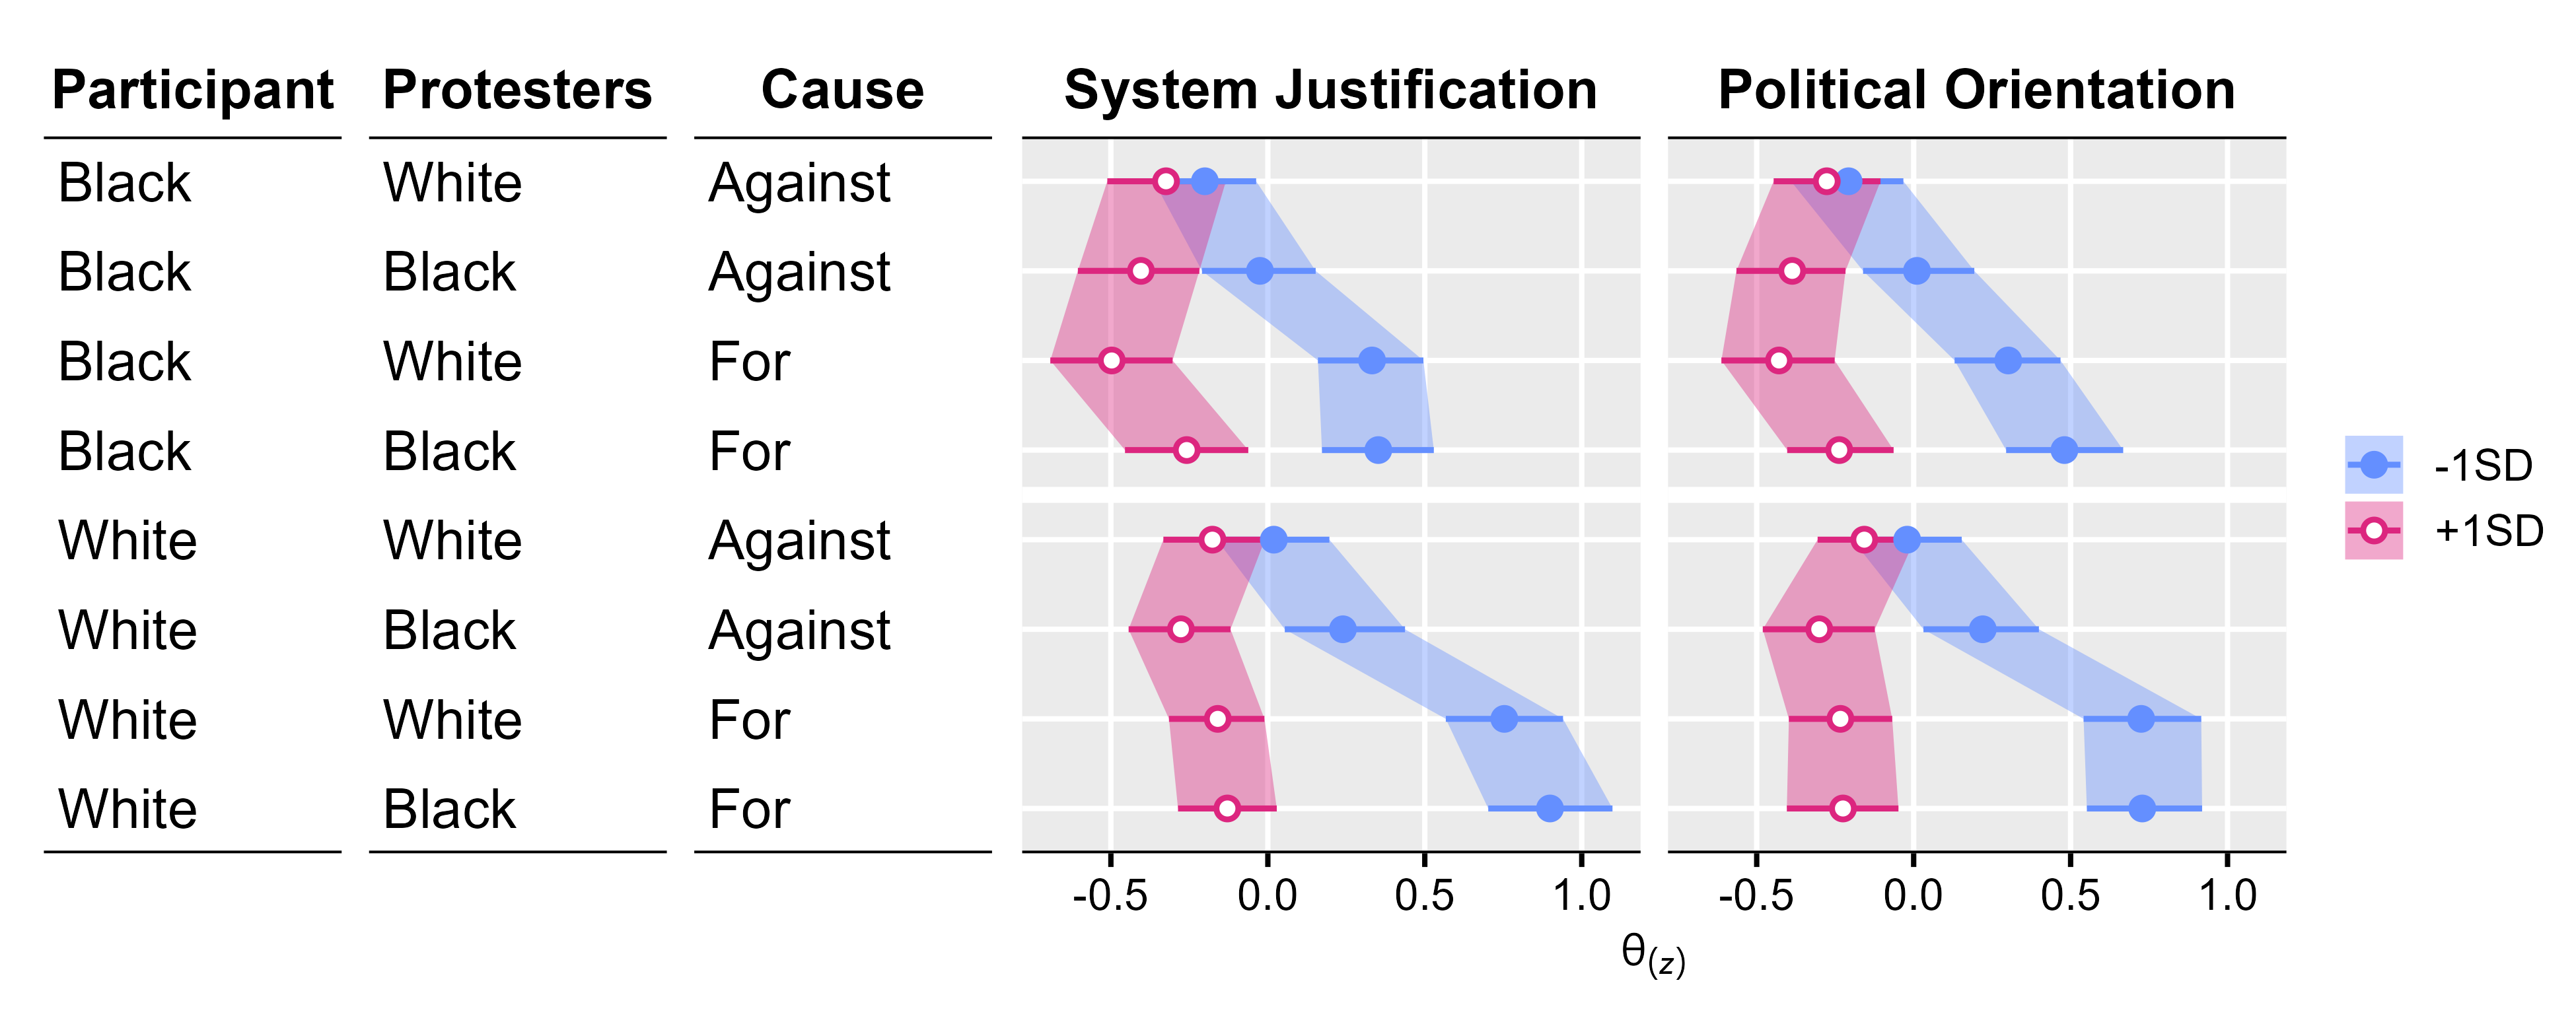
\includegraphics[scale=1]{../Experiment 2/figures/figure-s4}
\caption*{\textit{Note.} Against = Protesters oppose defunding the police. For = Protesters support defunding the police. $\theta_{(z)}$ is the \textit{z}-standardized tendency to consider more controversial actions acceptable means of protest.}
\label{fig:s4}
\end{figure*}

Figure \ref{fig:s3} shows results from three preregistered models we
estimated to test our hypotheses.

Model 1 estimated varying intercepts for the eight conditions to test
whether, in line with Hypotheses 1a, 1b, or 2a, participants' responses
depended on their own group membership, the protesters' group
membership, or the protesters' cause. Contradicting \emph{Hypothesis
1a}, participants did not consider protest actions performed by their
ingroup to be more acceptable, on average, than the same actions
performed by the relevant outgroup (\(d = 0.01, [-0.03, 0.06]\)).
Contradicting \emph{Hypothesis 1b}, participants did not consider
protest actions for a cause that was nominally aligned with their
ingroup's interests to be more acceptable, on average, than protest
actions for a cause not aligned with their ingroup's interests
(\(d = -0.01, [-0.06, 0.03]\)). Contradicting \emph{Hypothesis 2a},
participants did not consider protest actions for a system-defending
cause to be more acceptable, on average, than protest actions for a
system-challenging cause (\(d = -0.14, [-0.19, -0.08]\)). Instead, we
found that, on average, White participants considered all protest
actions to be more acceptable than Black participants
(\(d = 0.09, [0.04, 0.14]\)) and both Black (\(d = 0.12, [0.05, 0.19]\))
and White (\(d = 0.15, [0.08, 0.22]\)) participants considered the same
actions to be more acceptable when protests were for, rather than
against, defunding the police. As in Experiment 1, we thus found that
participants' responses depended on both the participants' and the
protesters' group memberships---but not in the directions predicted by
our hypotheses.

Model 2 extended Model 1 by estimating participants' responses as a
function of their \emph{z}-standardized endorsement of system-justifying
beliefs. As preregistered, we modeled this relationship with two fixed
effects, one estimating the effect of system-justifying beliefs on
judgments about system-defending protest actions and one estimating
their effect on judgments about system-challenging protest actions, and
one varying effect estimating its variance across conditions. Supporting
\emph{Hypothesis 2b}, participants who \emph{rejected} system-justifying
beliefs were \emph{more} likely to consider system-challenging protest
actions (for defunding the police) to be acceptable means of protest
(\(\beta_{xy} = 0.40, [0.20, 0.57]\)). We did not, however, find
evidence for the ideological symmetry implied by \emph{Hypothesis 2b}
since participants who \emph{endorsed} system-justifying beliefs were
\emph{not} more likely to consider system-defending protest actions
(against defunding the police) to be acceptable means of protest
(\(\beta_{xy} = -0.17, [-0.37, -0.01]\)).

Figure \ref{fig:s4} shows the estimated pattern of condition-wise
differences underlying those fixed effects. Participants who endorsed
system-justifying beliefs tended to consider system-challenging and
system-defending protest actions to be equally unacceptable. In
contrast, participants who rejected system-justifying beliefs evinced
ideology-based double standards: In line with \emph{Hypothesis 2b}, they
considered the same protest actions to be more acceptable when the
protesters challenged the system or, to a lesser extent, when the
protesters were from the disadvantaged group.

Model 3 extended Model 1 by estimating participants' responses as a
function of their self-reported support for the cause of the protest. We
recoded participants' responses to create a predictor variable that
encoded support for defunding the police when protesters supported
defunding the police and opposition to defunding the police when
protesters opposed defunding the police. As preregistered, we modeled
this relationship as a monotonic effect (Bürkner \& Charpentier, 2020)
that estimated the average change in the outcome variable across
predictor categories as well as how much of this change occurred between
each of the four pairs of adjacent predictor categories.\footnote{Our
  model assigned a Dirichlet prior, \(\alpha = {1, 1, 1, 1}\), to the
  proportions of the overall change that was expected to occur between
  each of the four pairs of predictor categories.} Contradicting
\emph{Hypothesis 3}, participants who supported the protesters' cause
did not, on average, consider the same protest actions to be more
acceptable than participants who opposed the protesters' cause
(\(\beta_{y} = 0.14, [-0.10, 0.39]\)). Ergo, our results did not support
the alternative hypothesis that ideology-based double standards can be
reduced to support for, or opposition to, the cause of a protest.

\hypertarget{non-preregistered-analyses}{%
\subsubsection{Non-Preregistered
Analyses}\label{non-preregistered-analyses}}

We explored whether group identification moderated how the participants'
and the protesters' group memberships affected participants' responses.
To that end, we extended Model 1 by estimating participants' responses
as a function of their \emph{z}-standardized identification with their
racial ingroup. As in Model 2, we modeled this relationship with a fixed
and a varying effect. We found, however, that even participants who
strongly identified with their racial ingroup (+1\emph{SD}) did not
consider protest actions performed by their ingroup to be more
acceptable than the same actions performed by the relevant outgroup
(\(d = 0.06, [-0.01, 0.13]\)) and did not consider protest actions for a
cause that was aligned with their ingroup's interests to be more
acceptable than protest actions for a cause not aligned with their
ingroup's interests (\(d = -0.00, [-0.07, 0.07]\)). Our
non-preregistered analyses thus suggested that group identification did
not moderate group differences in judgments about collective action by
ingroup and outgroup members.

We also explored whether we would find ideology-based double standards
when operationalizing ideology as political orientation instead of as
system justification. To that end, we reran Model 2 with political
orientation as the \emph{z}-standardized predictor variable. Our results
mirrored the preregistered analyses: More liberal participants were more
likely to consider protest actions for defunding the police to be
acceptable (\(\beta_{xy} = 0.40, [0.20, 0.58]\)) but more conservative
participants were not more likely to consider protest actions against
defunding the police to be acceptable
(\(\beta_{xy} = -0.16, [-0.35, 0.01]\)). As Figure \ref{fig:s4} shows,
conservative participants tended to consider all protest actions to be
equally unacceptable while liberal participants considered the same
protest actions to be more acceptable when protesters rallied around a
progressive cause. Our non-preregistered analyses thus replicated the
ideology-based double standards from the preregistered analyses with a
different operationalization of ideology.

\hypertarget{experiment-3-1}{%
\subsection{Experiment 3}\label{experiment-3-1}}

\begin{figure*}[!t]
\centering
\caption{Results from the preregistered analyses for Experiment 3 without exclusions}
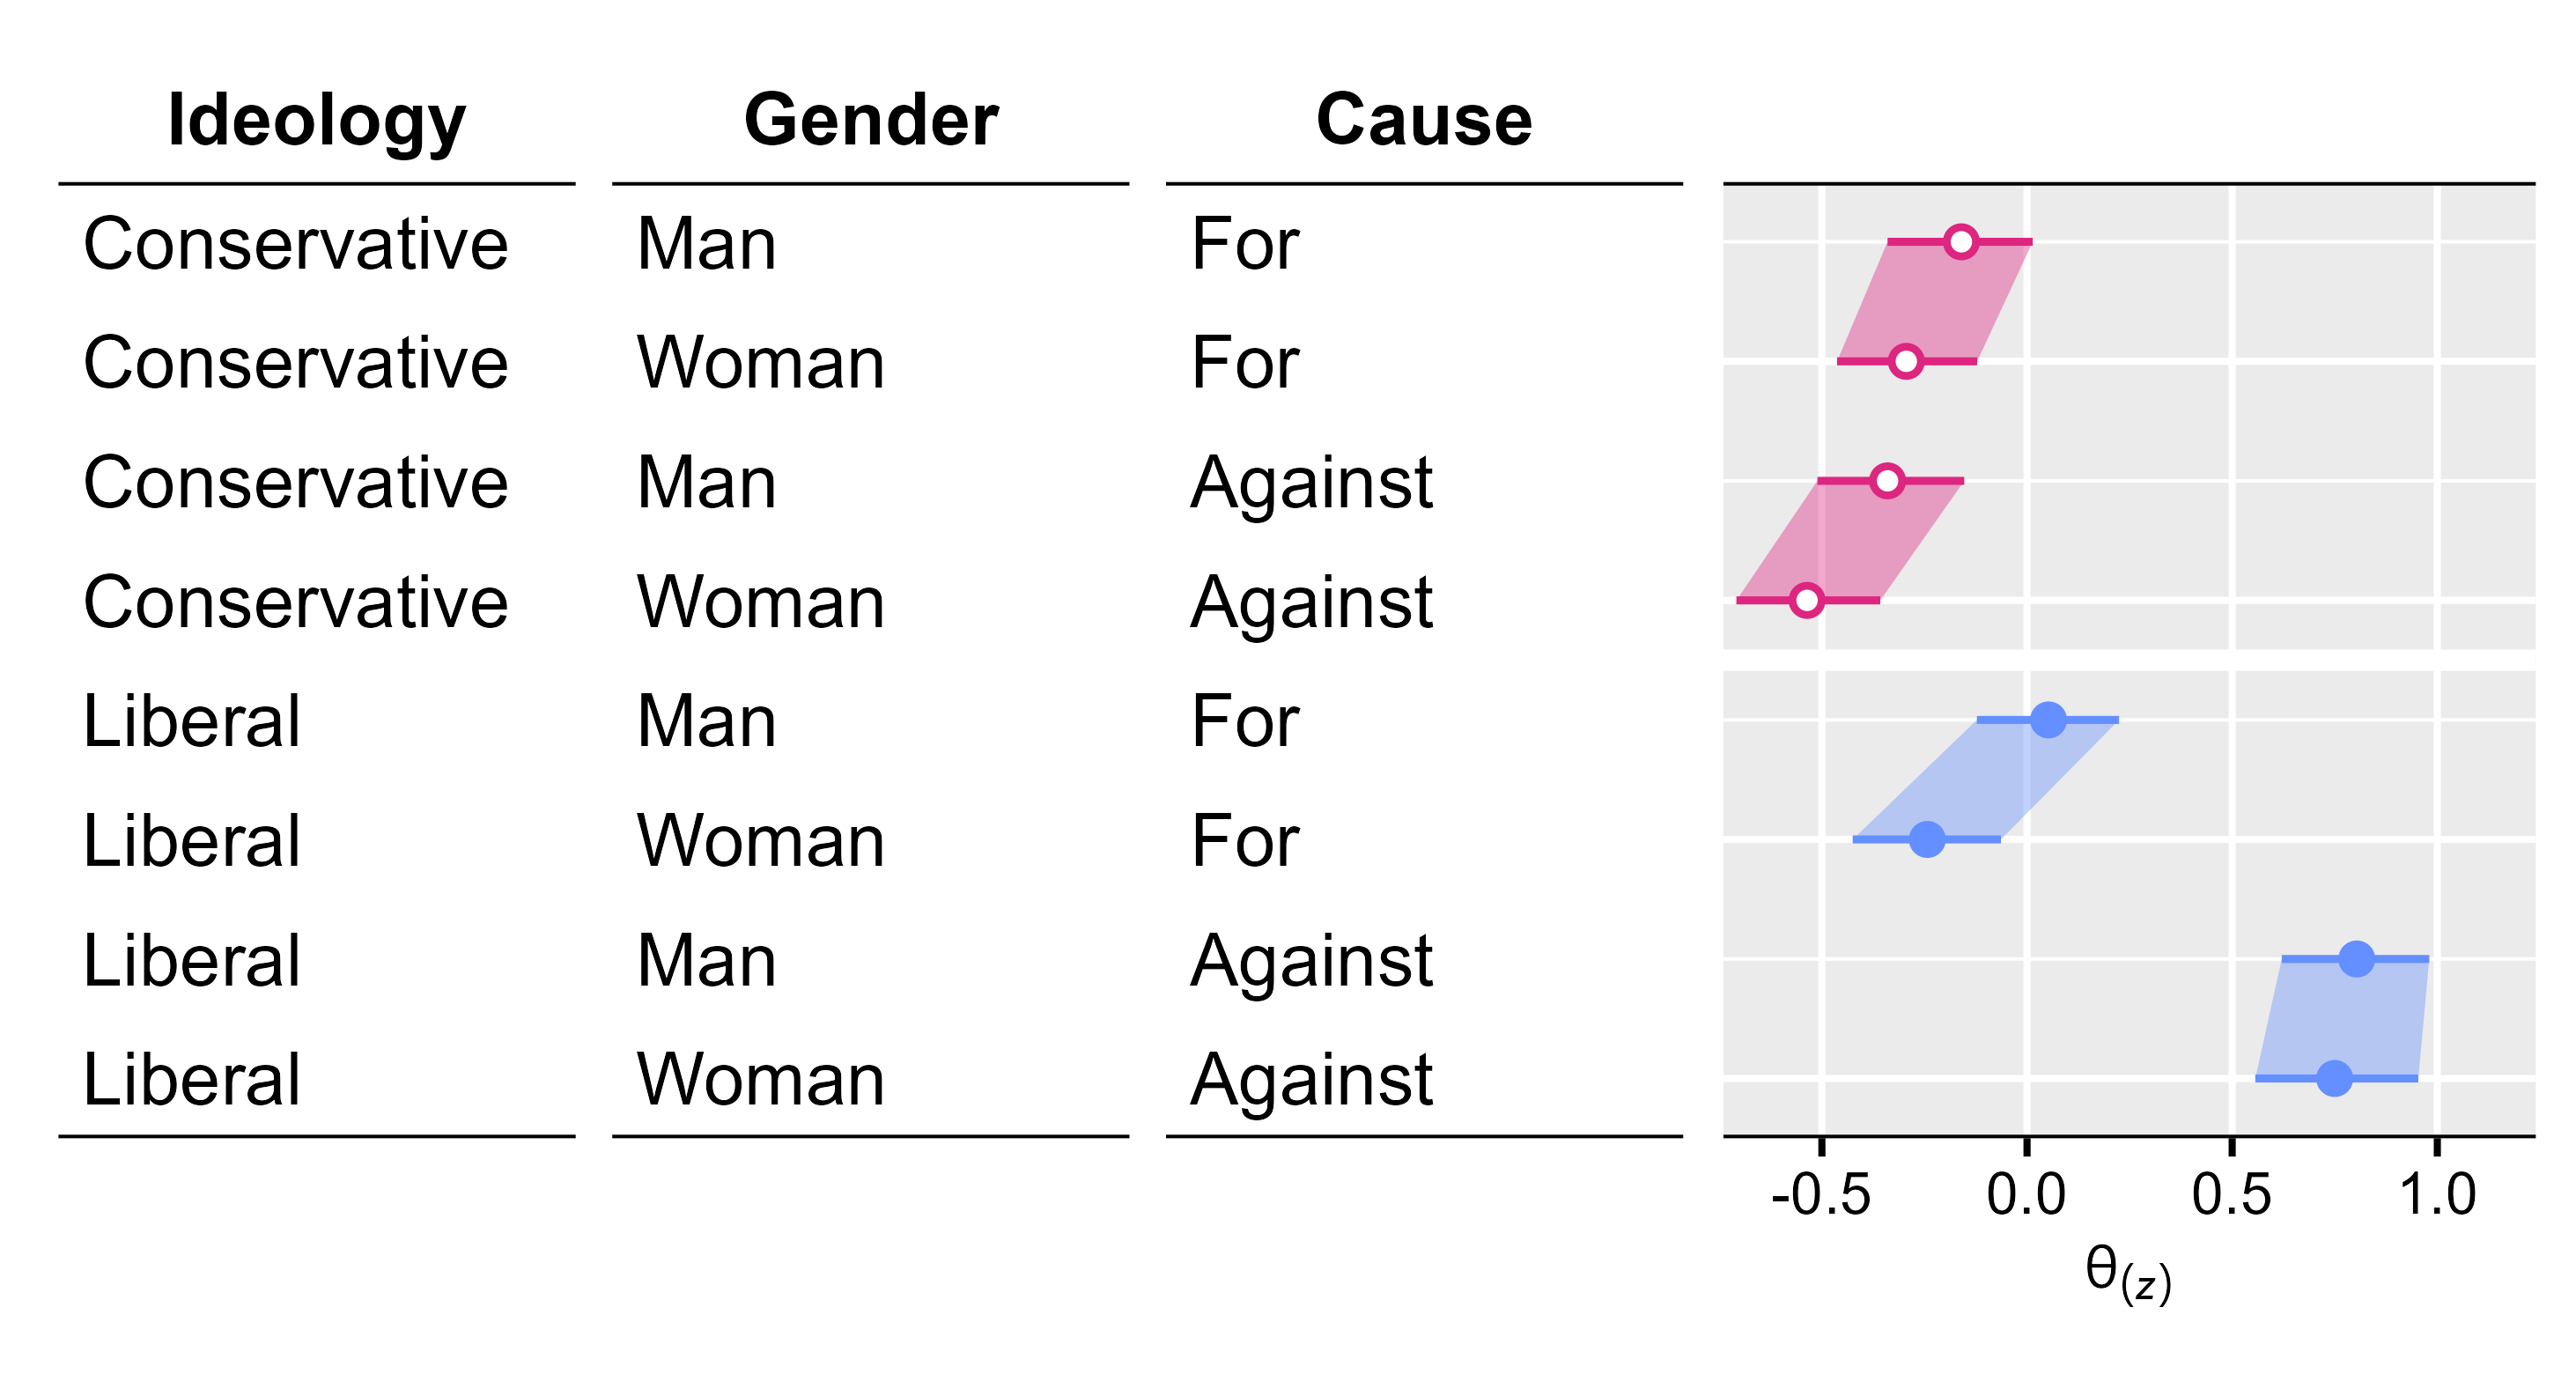
\includegraphics[scale=1]{../Experiment 3/figures/figure-s5}
\caption*{\textit{Note.} Results show the estimated \textit{z}-standardized tendency ($\theta_{(z)}$) to consider more controversial actions acceptable means to protest for or against restricting abortion as a function of the participants' ideology and gender.}
\label{fig:s5}
\end{figure*}

\hypertarget{preregistered-analyses-1}{%
\subsubsection{Preregistered Analyses}\label{preregistered-analyses-1}}

Figure \ref{fig:s5} shows the results of our preregistered analyses
without exclusions.

As in Experiments 1 and 2, we found evidence for ideology-based double
standards: Conservative participants considered the same protest actions
to be more acceptable, on average, when protesters \emph{supported}
restricting abortion (\(d = 0.21, [0.03, 0.39]\)) while liberal
participants considered the same protest actions to be more acceptable
when protesters \emph{opposed} restricting abortion
(\(d = 0.87, [0.70, 1.06]\)). This double standard was more pronounced
among liberal participants (\(d = 0.66, [0.42, 0.93]\)). In this way,
Experiment 3 provided evidence for both ideological symmetry and
asymmetry in judging collective action for and against restricting
abortion.

We found some evidence for identity-based double standards: Female
participants considered protest actions \emph{against} restricting
abortion to be more acceptable, on average, than male participants or
protest actions \emph{for} restricting abortion
(\(d = 0.14, [-0.01, 0.29]\)). This pattern was, however, overshadowed
by stronger ideology-based double standards that were consistent across
subsamples: Conservative women (\(d = 0.24, [-0.01, 0.48]\)) and, to a
lesser extent, conservative men (\(d = 0.18, [-0.08, 0.44]\)) considered
the same protest actions to be more acceptable when protesters
\emph{supported} restricting abortion and both liberal women
(\(d = 1.00, [0.73, 1.27]\)) and liberal men
(\(d = 0.75, [0.51, 1.01]\)) considered the same protest actions to be
more acceptable when protesters \emph{opposed} restricting abortion. In
this way, Experiment 3 provided more consistent evidence for
ideology-based than for identity-based double standards in judging
collective action.

\hypertarget{non-preregistered-analyses-1}{%
\subsubsection{Non-Preregistered
Analyses}\label{non-preregistered-analyses-1}}

We explored whether group identification moderated participants'
judgments. We found, however, that gender identification neither
affected how women judged protesters opposing
(\(\beta_{xy} = -0.06, [-0.15, 0.04]\)) or supporting
(\(\beta_{xy} = -0.07, [-0.16, 0.02]\)) abortion restrictions nor how
men judged protesters opposing (\(\beta_{xy} = -0.06, [-0.15, 0.03]\))
or supporting (\(\beta_{xy} = -0.06, [-0.14, 0.03]\)) abortion
restrictions. Our non-preregistered analyses thus suggested that gender
identification did not moderate identity-based double standards in
judging collective action concerning reproductive rights.

\newpage

\section*{References}

\begingroup

\noindent \setlength{\parindent}{-0.5in} \setlength{\leftskip}{0.5in}

\hypertarget{refs}{}
\begin{CSLReferences}{1}{0}
\leavevmode\vadjust pre{\hypertarget{ref-atari_morality_2023}{}}%
Atari, M., Haidt, J., Graham, J., Koleva, S., Stevens, S. T., \&
Dehghani, M. (2023). Morality beyond the {WEIRD}: {How} the nomological
network of morality varies across cultures. \emph{Journal of Personality
and Social Psychology}, \emph{125}(5), 1157--1188.
\url{https://doi.org/10.1037/pspp0000470}

\leavevmode\vadjust pre{\hypertarget{ref-betancourt_ordinal_2019}{}}%
Betancourt, M. (2019). \emph{Ordinal regression}.
\url{https://betanalpha.github.io/assets/case_studies/ordinal_regression.html}

\leavevmode\vadjust pre{\hypertarget{ref-burkner_bayesian_2021}{}}%
Bürkner, P.-C. (2021). Bayesian item response modeling in {R} with brms
and {Stan}. \emph{Journal of Statistical Software}, \emph{100}(5).
\url{https://doi.org/10.18637/jss.v100.i05}

\leavevmode\vadjust pre{\hypertarget{ref-burkner_modelling_2020}{}}%
Bürkner, P.-C., \& Charpentier, E. (2020). Modelling monotonic effects
of ordinal predictors in {Bayesian} regression models. \emph{British
Journal of Mathematical and Statistical Psychology}, \emph{73}(3),
420--451. \url{https://doi.org/10.1111/bmsp.12195}

\leavevmode\vadjust pre{\hypertarget{ref-jost_exposure_2005}{}}%
Jost, J. T., \& Kay, A. C. (2005). Exposure to benevolent sexism and
complementary gender stereotypes: Consequences for specific and diffuse
forms of system justification. \emph{Journal of Personality and Social
Psychology}, \emph{88}(3), 498--509.
\url{https://doi.org/10.1037/0022-3514.88.3.498}

\leavevmode\vadjust pre{\hypertarget{ref-ryan_reconsidering_2014}{}}%
Ryan, T. J. (2014). Reconsidering moral issues in politics. \emph{The
Journal of Politics}, \emph{76}(2), 380--397.
\url{https://doi.org/10.1017/S0022381613001357}

\leavevmode\vadjust pre{\hypertarget{ref-samejima_graded_1997}{}}%
Samejima, F. (1997). Graded response model. In W. J. van der Linden \&
R. K. Hambleton (Eds.), \emph{Handbook of modern item response theory}
(pp. 85--100). Springer.

\leavevmode\vadjust pre{\hypertarget{ref-sharp_nonviolent_1973}{}}%
Sharp, G. (1973). \emph{The politics of nonviolent action}. Porter
Sargent.

\end{CSLReferences}

\endgroup

\newpage

\begin{xltabular}{\linewidth}{rXrrrrrrr}

\caption{Results from Study 2}\\
\toprule
   &        &     &          & \multicolumn{5}{c}{Response $[\%]$} \\ \cmidrule{5-9}
\# & Action & $I$ & $\alpha$ & 1 & 2 & 3 & 4 & 5\\
\midrule
\endfirsthead

\toprule
   &        &     &          & \multicolumn{5}{c}{Response $[\%]$} \\ \cmidrule{5-9}
\# & Action & $I$ & $\alpha$ & 1 & 2 & 3 & 4 & 5\\
\midrule
\endhead

\bottomrule
\addlinespace
\caption*{\textit{Note.} $I$ = Information; $\alpha$ = Discrimination; Response: 1 = \textit{never}, 2 = \textit{rarely}, 3 = \textit{sometimes}, 4 = \textit{often}, 5 = \textit{always}}
\endfoot

\bottomrule
\addlinespace
\caption*{\textit{Note.} $I$ = Information; $\alpha$ = Discrimination; Response: 1 = \textit{never}, 2 = \textit{rarely}, 3 = \textit{sometimes}, 4 = \textit{often}, 5 = \textit{always}}
\endlastfoot

1 & disrupt traffic (e.g., blocking roads) & 7.98 & 1.31 & 41 & 36 & 18 & 5 & 0\\
2 & attend or organise a protest rally & 7.35 & 1.11 & 0 & 7 & 45 & 39 & 9\\
3 & refuse to work (strike) & 6.96 & 1.11 & 2 & 5 & 53 & 33 & 7\\
4 & enter and refuse to leave a building (occupation) & 6.95 & 1.12 & 6 & 52 & 26 & 13 & 3\\
5 & deface flags or other national symbols & 6.83 & 1.21 & 52 & 20 & 20 & 9 & 0\\

6 & refuse to honour national symbols and traditions (e.g., refusing to sing the national anthem) & 6.42 & 1.19 & 15 & 18 & 40 & 15 & 12\\
7 & paste up posters with political messages in places where it is not allowed or encouraged & 6.37 & 1.01 & 14 & 32 & 35 & 19 & 0\\
8 & refuse to cooperate with the police and other government agencies & 6.37 & 1.11 & 22 & 38 & 32 & 5 & 3\\
9 & refuse to accept honours or awards in protest & 6.32 & 1.14 & 11 & 14 & 39 & 23 & 14\\
10 & disrupt public events (e.g., a sports game) with a political message & 6.30 & 1.02 & 24 & 45 & 21 & 10 & 0\\

11 & spray paint political messages in public places & 6.28 & 1.06 & 31 & 39 & 28 & 3 & 0\\
12 & stand or sit in a building and refuse to leave (stand-in, sit-in) & 6.28 & 1.04 & 7 & 41 & 34 & 14 & 5\\
13 & pay for adverts on social media (e.g., Facebook, Twitter, Instagram) to influence public opinion & 6.23 & 0.99 & 0 & 16 & 27 & 39 & 18\\
14 & get involved in the media (e.g., newspapers, radio, television) to influence the public & 6.18 & 0.98 & 0 & 11 & 32 & 36 & 20\\
15 & visit people in their homes to convince them about an issue (canvassing, door knocking) & 6.07 & 1.03 & 9 & 30 & 27 & 27 & 6\\

16 & donate to political parties who support the cause & 6.00 & 1.10 & 6 & 6 & 33 & 31 & 25\\
17 & do not buy goods or services from companies who oppose the cause (consumers' boycott) & 5.99 & 1.06 & 2 & 5 & 39 & 29 & 24\\
18 & refuse to interact with or acknowledge individuals who oppose the cause & 5.89 & 0.97 & 21 & 45 & 29 & 5 & 0\\
19 & attend or organise a protest march & 5.88 & 1.06 & 3 & 3 & 34 & 38 & 22\\
20 & paste up posters with political messages in places where it is allowed and encouraged & 5.85 & 1.00 & 0 & 3 & 20 & 43 & 34\\

21 & refuse to pay rent (rent strike) & 5.82 & 0.97 & 23 & 41 & 28 & 8 & 0\\
22 & use social media (e.g., Facebook, Twitter, Instagram) to influence the public & 5.82 & 1.01 & 5 & 5 & 30 & 45 & 15\\
23 & wear or display political symbols & 5.79 & 1.00 & 3 & 9 & 38 & 32 & 18\\
24 & mock or insult individuals who oppose the cause & 5.73 & 1.11 & 53 & 34 & 3 & 11 & 0\\
25 & write letters to politicians, representatives and elected officials & 5.69 & 1.07 & 0 & 0 & 11 & 37 & 53\\

26 & use social media (e.g., Facebook, Twitter, Instagram) to inform the public & 5.67 & 1.01 & 0 & 3 & 12 & 41 & 44\\
27 & join or form a group of activists & 5.66 & 1.02 & 2 & 12 & 21 & 38 & 26\\
28 & hold meetings to inform the public & 5.65 & 1.01 & 0 & 3 & 11 & 38 & 49\\
29 & donate to activist groups who support the cause & 5.64 & 1.06 & 2 & 9 & 41 & 14 & 34\\
30 & disrupt public services (e.g., shutting down government websites) & 5.61 & 1.01 & 42 & 42 & 17 & 0 & 0\\

31 & refuse to pay fees, fines, and taxes & 5.56 & 0.96 & 9 & 50 & 30 & 7 & 4\\
32 & hold meetings to influence the public & 5.56 & 1.00 & 0 & 3 & 16 & 35 & 46\\
33 & hand out flyers, leaflets, or pamphlets & 5.55 & 1.01 & 0 & 0 & 13 & 45 & 42\\
34 & visit people in their homes to inform them about an issue (canvassing, door knocking) & 5.39 & 0.95 & 9 & 20 & 30 & 32 & 9\\
35 & make a public speech & 5.35 & 1.00 & 2 & 2 & 14 & 46 & 36\\

36 & join or form a political party & 5.28 & 0.96 & 2 & 7 & 19 & 45 & 26\\
37 & refuse to interact with or acknowledge politicians who oppose the cause & 5.27 & 0.95 & 8 & 35 & 38 & 10 & 10\\
38 & disrupt private life of politicians (e.g., protesting outside their home) & 5.24 & 0.92 & 39 & 36 & 23 & 2 & 0\\
39 & get involved in the media (e.g., newspapers, radio, television) to inform the public & 5.23 & 0.93 & 0 & 2 & 11 & 43 & 43\\
40 & pay for adverts in the media (e.g., newspapers, radio, television) to influence public opinion & 5.23 & 0.97 & 5 & 10 & 22 & 42 & 20\\

41 & damage private property (e.g., cars or houses) & 5.17 & 1.03 & 70 & 25 & 5 & 0 & 0\\
42 & refuse service (e.g., in a restaurant or shop) to politicians who oppose the cause & 5.16 & 0.89 & 29 & 37 & 26 & 8 & 0\\
43 & sign or start a petition & 5.10 & 0.96 & 0 & 0 & 8 & 39 & 53\\
44 & mock or insult politicians who oppose the cause & 5.07 & 0.99 & 38 & 31 & 16 & 11 & 4\\
45 & join or form a trade/labor union & 5.07 & 0.99 & 2 & 2 & 14 & 37 & 44\\

46 & donate to charities who support the cause & 5.03 & 0.96 & 0 & 0 & 8 & 39 & 53\\
47 & refuse to eat (hunger strike) & 4.95 & 0.97 & 38 & 24 & 29 & 6 & 3\\
48 & damage public property (e.g., goverment buildings) & 4.83 & 0.98 & 72 & 20 & 5 & 2 & 0\\
49 & spread rumours about politicians who oppose the cause & 4.77 & 1.00 & 69 & 21 & 10 & 0 & 0\\
50 & participate in a public meeting of representatives and elected officials & 4.70 & 1.00 & 3 & 0 & 7 & 47 & 43\\

51 & physically harm oneself (e.g., setting oneself on fire) & 4.70 & 1.03 & 80 & 20 & 0 & 0 & 0\\
52 & boycott an election by not voting or spoiling one's ballot & 4.70 & 0.91 & 14 & 38 & 26 & 12 & 10\\
53 & stand in an election & 4.69 & 0.90 & 2 & 8 & 18 & 35 & 38\\
54 & soil politicians who oppose the cause (e.g., throwing eggs at them) & 4.62 & 1.02 & 70 & 21 & 8 & 0 & 2\\
55 & attack politicians with the intention of harming them (e.g., punching them) & 4.62 & 1.01 & 78 & 22 & 0 & 0 & 0\\

56 & refuse service (e.g., in a restaurant or shop) to individuals who oppose the cause & 4.60 & 0.91 & 32 & 54 & 11 & 0 & 3\\
57 & blackmail individuals who oppose the cause & 4.53 & 0.96 & 75 & 22 & 3 & 0 & 0\\
58 & threaten politicians who oppose the cause with physical harm & 4.37 & 1.00 & 86 & 11 & 3 & 0 & 0\\
59 & attack individuals who oppose the cause with the intention of harming them (e.g., punching them) & 4.36 & 0.95 & 82 & 12 & 6 & 0 & 0\\
60 & damage commerical property (e.g., shop windows) & 4.36 & 1.03 & 88 & 12 & 0 & 0 & 0\\

61 & attack politicians with the intention of killing them (e.g., stabbing them) & 4.30 & 1.01 & 91 & 7 & 2 & 0 & 0\\
62 & bribe politicians, representatives, and other elected officials & 4.24 & 0.95 & 85 & 13 & 2 & 0 & 0\\
63 & voting for candidates/parties & 4.23 & 0.85 & 0 & 5 & 7 & 21 & 67\\
64 & donate to political parties to make them change their position on an issue & 4.21 & 0.90 & 35 & 24 & 30 & 3 & 8\\
65 & blackmail politicians who oppose the cause & 4.20 & 0.88 & 72 & 26 & 3 & 0 & 0\\

66 & attack police officers and other government agents with the intention of killing them (e.g., stabbing them) & 4.20 & 1.02 & 93 & 7 & 0 & 0 & 0\\
67 & attack police officers and other government agents with the intention of harming them (e.g., punching them) & 4.17 & 1.00 & 92 & 5 & 3 & 0 & 0\\
68 & attack individuals who oppose the cause with the intention of killing them (e.g., stabbing them) & 3.98 & 1.00 & 96 & 2 & 2 & 0 & 0\\
69 & threaten individuals who oppose the cause with physical harm & 3.96 & 0.99 & 94 & 6 & 0 & 0 & 0\\
70 & attack members of the public (e.g., by setting off a bomb in a public place) & 3.72 & 0.99 & 98 & 0 & 2 & 0 & 0\\

71 & spread misinformation to influence public opinion & 3.71 & 0.82 & 78 & 19 & 3 & 0 & 0\\
72 & threaten to attack members of the public (e.g., by making a bomb threat) & 3.51 & 0.97 & 98 & 0 & 0 & 2 & 0

\end{xltabular}

\newpage

\setcounter{table}{1}

\begin{xltabular}{\linewidth}{rXrrrrr}

\caption{Ratings from Study 2}\\
\toprule
   &        & \multicolumn{5}{c}{Rating $[M]$} \\ \cmidrule{3-7}
\# & Action & Acce. & Disr. & Viol. & Extr. & Nega.\\
\midrule
\endfirsthead

\toprule
   &        & \multicolumn{5}{c}{Rating $[M]$} \\ \cmidrule{3-7}
\# & Action & Acce. & Disr. & Viol. & Extr. & Nega.\\
\midrule
\endhead

\bottomrule
\addlinespace
\caption*{\textit{Note.} Acce. = Acceptable (1 = \textit{never}, 5 = \textit{always}); Disr. = Disruptive, Viol. = Violent, Extr. = Extreme (1 = \textit{not at all}, 4 = \textit{very}); Nega. = Negative (1 = \textit{very positive}, 5 = \textit{very negative})}
\endfoot

\bottomrule
\addlinespace
\caption*{\textit{Note.} Acce. = Acceptable (1 = \textit{never}, 5 = \textit{always}); Disr. = Disruptive, Viol. = Violent, Extr. = Extreme (1 = \textit{not at all}, 4 = \textit{very}); Nega. = Negative (1 = \textit{very positive}, 5 = \textit{very negative})}
\endlastfoot

1 & disrupt traffic (e.g., blocking roads) & 1.86 & 3.82 & 2.05 & 2.98 & 4.16\\
2 & attend or organise a protest rally & 3.50 & 2.50 & 1.36 & 1.48 & 2.64\\
3 & refuse to work (strike) & 3.37 & 3.35 & 1.09 & 2.07 & 2.60\\
4 & enter and refuse to leave a building (occupation) & 2.55 & 3.32 & 1.48 & 2.42 & 3.19\\
5 & deface flags or other national symbols & 1.85 & 2.98 & 2.30 & 2.98 & 4.15\\

6 & refuse to honour national symbols and traditions (e.g., refusing to sing the national anthem) & 2.92 & 1.85 & 1.23 & 1.62 & 3.20\\
7 & paste up posters with political messages in places where it is not allowed or encouraged & 2.59 & 2.84 & 1.22 & 1.92 & 3.38\\
8 & refuse to cooperate with the police and other government agencies & 2.30 & 3.14 & 2.11 & 2.78 & 3.76\\
9 & refuse to accept honours or awards in protest & 3.14 & 1.84 & 1.07 & 1.59 & 2.86\\
10 & disrupt public events (e.g., a sports game) with a political message & 2.17 & 3.40 & 1.60 & 2.31 & 3.79\\

11 & spray paint political messages in public places & 2.03 & 2.72 & 1.53 & 2.44 & 3.97\\
12 & stand or sit in a building and refuse to leave (stand-in, sit-in) & 2.68 & 3.34 & 1.27 & 2.16 & 3.02\\
13 & pay for adverts on social media (e.g., Facebook, Twitter, Instagram) to influence public opinion & 3.59 & 1.59 & 1.02 & 1.30 & 2.75\\
14 & get involved in the media (e.g., newspapers, radio, television) to influence the public & 3.66 & 1.61 & 1.02 & 1.23 & 2.41\\
15 & visit people in their homes to convince them about an issue (canvassing, door knocking) & 2.91 & 2.76 & 1.06 & 1.36 & 3.33\\

16 & donate to political parties who support the cause & 3.64 & 1.14 & 1.00 & 1.17 & 2.47\\
17 & do not buy goods or services from companies who oppose the cause (consumers' boycott) & 3.68 & 2.07 & 1.05 & 1.29 & 2.27\\
18 & refuse to interact with or acknowledge individuals who oppose the cause & 2.18 & 2.42 & 1.24 & 2.37 & 3.79\\
19 & attend or organise a protest march & 3.72 & 2.56 & 1.31 & 1.56 & 2.41\\
20 & paste up posters with political messages in places where it is allowed and encouraged & 4.09 & 1.31 & 1.00 & 1.06 & 2.17\\

21 & refuse to pay rent (rent strike) & 2.21 & 2.72 & 1.10 & 2.41 & 3.67\\
22 & use social media (e.g., Facebook, Twitter, Instagram) to influence the public & 3.60 & 1.40 & 1.00 & 1.15 & 2.42\\
23 & wear or display political symbols & 3.53 & 1.29 & 1.03 & 1.09 & 2.71\\
24 & mock or insult individuals who oppose the cause & 1.71 & 2.79 & 1.95 & 2.58 & 4.18\\
25 & write letters to politicians, representatives and elected officials & 4.42 & 1.39 & 1.05 & 1.03 & 1.53\\

26 & use social media (e.g., Facebook, Twitter, Instagram) to inform the public & 4.25 & 1.31 & 1.00 & 1.06 & 2.03\\
27 & join or form a group of activists & 3.74 & 1.81 & 1.38 & 1.50 & 2.38\\
28 & hold meetings to inform the public & 4.32 & 1.19 & 1.00 & 1.03 & 1.81\\
29 & donate to activist groups who support the cause & 3.68 & 1.39 & 1.11 & 1.25 & 2.39\\
30 & disrupt public services (e.g., shutting down government websites) & 1.75 & 3.75 & 1.61 & 3.06 & 4.28\\

31 & refuse to pay fees, fines, and taxes & 2.48 & 2.61 & 1.04 & 2.09 & 3.46\\
32 & hold meetings to influence the public & 4.24 & 1.14 & 1.00 & 1.03 & 1.86\\
33 & hand out flyers, leaflets, or pamphlets & 4.29 & 1.47 & 1.03 & 1.05 & 2.00\\
34 & visit people in their homes to inform them about an issue (canvassing, door knocking) & 3.11 & 2.45 & 1.07 & 1.50 & 3.16\\
35 & make a public speech & 4.12 & 1.46 & 1.00 & 1.06 & 1.92\\

36 & join or form a political party & 3.86 & 1.40 & 1.00 & 1.24 & 2.10\\
37 & refuse to interact with or acknowledge politicians who oppose the cause & 2.80 & 1.88 & 1.15 & 1.88 & 3.52\\
38 & disrupt private life of politicians (e.g., protesting outside their home) & 1.89 & 3.36 & 2.07 & 2.77 & 4.07\\
39 & get involved in the media (e.g., newspapers, radio, television) to inform the public & 4.27 & 1.36 & 1.02 & 1.14 & 1.82\\
40 & pay for adverts in the media (e.g., newspapers, radio, television) to influence public opinion & 3.62 & 1.60 & 1.10 & 1.35 & 2.50\\

41 & damage private property (e.g., cars or houses) & 1.34 & 3.77 & 3.64 & 3.86 & 4.75\\
42 & refuse service (e.g., in a restaurant or shop) to politicians who oppose the cause & 2.13 & 2.95 & 1.26 & 2.39 & 3.71\\
43 & sign or start a petition & 4.45 & 1.18 & 1.03 & 1.03 & 1.74\\
44 & mock or insult politicians who oppose the cause & 2.13 & 2.31 & 1.58 & 2.02 & 3.84\\
45 & join or form a trade/labor union & 4.19 & 1.40 & 1.00 & 1.07 & 1.70\\

46 & donate to charities who support the cause & 4.44 & 1.03 & 1.00 & 1.03 & 1.47\\
47 & refuse to eat (hunger strike) & 2.12 & 2.26 & 1.38 & 3.32 & 3.74\\
48 & damage public property (e.g., goverment buildings) & 1.38 & 3.67 & 3.55 & 3.65 & 4.68\\
49 & spread rumours about politicians who oppose the cause & 1.41 & 3.14 & 1.72 & 2.76 & 4.31\\
50 & participate in a public meeting of representatives and elected officials & 4.27 & 1.23 & 1.07 & 1.07 & 1.80\\

51 & physically harm oneself (e.g., setting oneself on fire) & 1.20 & 3.68 & 3.76 & 3.95 & 4.83\\
52 & boycott an election by not voting or spoiling one's ballot & 2.64 & 2.24 & 1.19 & 1.90 & 3.45\\
53 & stand in an election & 3.98 & 1.27 & 1.02 & 1.15 & 1.98\\
54 & soil politicians who oppose the cause (e.g., throwing eggs at them) & 1.43 & 3.28 & 3.11 & 3.19 & 4.47\\
55 & attack politicians with the intention of harming them (e.g., punching them) & 1.22 & 3.65 & 3.81 & 3.84 & 4.81\\

56 & refuse service (e.g., in a restaurant or shop) to individuals who oppose the cause & 1.86 & 3.03 & 1.46 & 2.65 & 4.16\\
57 & blackmail individuals who oppose the cause & 1.28 & 3.33 & 2.56 & 3.61 & 4.72\\
58 & threaten politicians who oppose the cause with physical harm & 1.16 & 3.57 & 3.76 & 3.81 & 4.81\\
59 & attack individuals who oppose the cause with the intention of harming them (e.g., punching them) & 1.24 & 3.76 & 3.88 & 3.88 & 4.79\\
60 & damage commerical property (e.g., shop windows) & 1.12 & 3.85 & 3.79 & 3.79 & 4.91\\

61 & attack politicians with the intention of killing them (e.g., stabbing them) & 1.11 & 3.93 & 4.00 & 4.00 & 4.91\\
62 & bribe politicians, representatives, and other elected officials & 1.17 & 3.02 & 1.28 & 3.04 & 4.85\\
63 & voting for candidates/parties & 4.51 & 1.19 & 1.09 & 1.07 & 1.63\\
64 & donate to political parties to make them change their position on an issue & 2.24 & 2.03 & 1.05 & 1.68 & 3.68\\
65 & blackmail politicians who oppose the cause & 1.31 & 3.15 & 2.15 & 3.54 & 4.64\\

66 & attack police officers and other government agents with the intention of killing them (e.g., stabbing them) & 1.07 & 4.00 & 4.00 & 4.00 & 4.98\\
67 & attack police officers and other government agents with the intention of harming them (e.g., punching them) & 1.11 & 3.81 & 3.95 & 3.95 & 4.95\\
68 & attack individuals who oppose the cause with the intention of killing them (e.g., stabbing them) & 1.06 & 3.94 & 4.00 & 4.00 & 4.92\\
69 & threaten individuals who oppose the cause with physical harm & 1.06 & 3.72 & 3.92 & 3.97 & 4.92\\
70 & attack members of the public (e.g., by setting off a bomb in a public place) & 1.05 & 3.90 & 3.92 & 3.92 & 4.92\\

71 & spread misinformation to influence public opinion & 1.24 & 3.41 & 1.41 & 2.95 & 4.76\\
72 & threaten to attack members of the public (e.g., by making a bomb threat) & 1.07 & 3.83 & 3.83 & 3.85 & 4.95

\end{xltabular}

\newpage

\setcounter{table}{2}

\begin{table}[t!]
\caption{Correlations between ratings in Study 2}
\centering
\begin{tabular}{rlrrrrr}
\toprule
\# & Rating & Acceptable & Disruptive & Violent & Extreme & Negative\\
\midrule1 & Acceptable &  & -.69 & -.64 & -.77 & -.89\\
2 & Disruptive & -.69 &  & .66 & .78 & .70\\
3 & Violent & -.64 & .66 &  & .79 & .64\\
4 & Extreme & -.77 & .78 & .79 &  & .77\\
5 & Negative & -.89 & .70 & .64 & .77 & \\
\bottomrule
\addlinespace
\end{tabular}
\caption*{\textit{Note.} Acceptable (1 = \textit{never}, 5 = \textit{always}); Disruptive, Violent, Extreme (1 = \textit{not at all}, 4 = \textit{very}); Negative (1 = \textit{very positive}, 5 = \textit{very negative})}
\end{table}

\setcounter{table}{3}

\begin{table}[t!]
\caption{Correlations between variables in Experiment 1}
\centering
\begin{tabular}{rlrrrr}
\toprule
\# & Variable              &    1 &    2 &    3 &    4 \\ \midrule
 1 & Proportion            &      & -.31 & -.16 & -.23 \\
 2 & Political Orientation & -.31 &      &  .41 &  .41 \\
 3 & Social Dominance      & -.16 &  .41 &      &  .29 \\
 4 & System Justification  & -.23 &  .41 &  .29 &      \\ \bottomrule
\addlinespace
\end{tabular}
\caption*{\textit{Note.} Proportion of actions considered acceptable (0--1); Political Orientation (1 = \textit{left}, 7 = \textit{right}); Social Dominance Orientation (\textit{factor score}); System-Justifying Beliefs (\textit{factor score})}
\end{table}

\setcounter{table}{4}

\begin{table}[t!]
\caption{Correlations between variables in Experiment 2}
\centering
\begin{tabular}{rlrrrrr}
\toprule
\# & Variable              &    1 &    2 &    3 &    4 &    5 \\ \midrule
 1 & Proportion            &      & -.21 &  .29 & -.23 & -.07 \\
 2 & System Justification  & -.21 &      & -.45 &  .47 &  .04 \\
 3 & Policy Support        &  .29 & -.45 &      & -.49 &  .00 \\
 4 & Political Orientation & -.23 &  .47 & -.49 &      &  .03 \\
 5 & Identification        & -.07 &  .04 &  .00 &  .03 &      \\ \bottomrule
\addlinespace
\end{tabular}
\caption*{\textit{Note.} Proportion of actions considered acceptable (0--1); System-Justifying Beliefs (\textit{factor score}); Policy Support (1 = \textit{strongly oppose}, 5 = \textit{strongly support}); Political Orientation (1 = \textit{liberal}, 7 = \textit{conservative}); Racial Identification (1 = \textit{not at all}, 7 = \textit{very much})}
\end{table}

\setcounter{table}{5}

\begin{table}[t!]
\caption{Correlations between variables in Experiment 3}
\centering
\begin{tabular}{rlrrrrr}
\toprule
\# & Variable              &    1 &    2 &    3 &    4 &    5 \\ \midrule
 1 & Proportion            &      & -.27 & -.22 & -.32 & -.11 \\
 2 & System Justification  & -.27 &      &  .61 &  .78 &  .16 \\
 3 & Policy Support        & -.22 &  .61 &      &  .74 &  .16 \\
 4 & Political Orientation & -.32 &  .78 &  .74 &      &  .20 \\
 5 & Identification        & -.11 &  .16 &  .16 &  .20 &      \\ \bottomrule
\addlinespace
\end{tabular}
\caption*{\textit{Note.} Proportion of actions considered acceptable (0--1); System-Justifying Beliefs (\textit{factor score}); Policy Support (1 = \textit{strongly oppose}, 5 = \textit{strongly support}); Political Orientation (1 = \textit{liberal}, 7 = \textit{conservative}); Gender Identification (1 = \textit{not at all}, 7 = \textit{very much})}
\end{table}

\end{document}
